\documentclass[11pt,a4paper]{article}

% ---------- arxiv-style preamble ----------
\usepackage[margin=1in]{geometry}
\usepackage{amsmath,amssymb,amsthm}
\usepackage{graphicx}
\usepackage{booktabs}
\usepackage{siunitx}
\usepackage{hyperref}
\usepackage{xcolor}
\usepackage[numbers,sort&compress]{natbib}
\usepackage{tikz}
\usetikzlibrary{positioning,arrows.meta}
\usepackage{caption}
\usepackage{listings}
\usepackage{array}
\captionsetup{font=small,labelfont=bf}
\hypersetup{
  colorlinks=true,
  linkcolor=blue!50!black,
  citecolor=blue!50!black,
  urlcolor=blue!50!black
}

% ---------- emoji tier badges (xelatex-native; pdflatex must use replacement marks) ----------
% Use \tierBlue / \tierGreen / \tierYellow / \tierOrange / \tierRed in tables so
% the source stays compile-safe under either engine. Default = literal emoji
% (xelatex/lualatex render natively; the shipped Makefile pins xelatex).
\providecommand{\tierBlue}{🔵}
\providecommand{\tierGreen}{🟢}
\providecommand{\tierYellow}{🟡}
\providecommand{\tierOrange}{🟠}
\providecommand{\tierRed}{🔴}

\title{
  \textbf{TITLE HERE}\\[4pt]
  \large SUBTITLE OR FRAMING
}

% ---------- author block (hexa-codex style) ----------
% Convention: <repo> maintainers / dancinlab / clickable github URL.
% LLM collaborator goes in \paragraph{Acknowledgments} at the tail — NOT here.
\author{
  \texttt{<repo>} maintainers\\
  \normalsize\textit{dancinlab}\\[2pt]
  \normalsize\href{https://github.com/dancinlab/<repo>}{\texttt{github.com/dancinlab/<repo>}}
}

\date{\today}

\begin{document}

\maketitle

% =========================================================================
\begin{abstract}
One-paragraph abstract. State the question, the method, the headline
result with the smallest numeric quantity that makes it falsifiable,
and one sentence on scope / what is \emph{not} claimed. Close with a
pointer to the \texttt{companion/} data records (verify-ledger,
PR-roll, session journal) for bit-for-bit reproduction.
\end{abstract}

\section{Introduction}
\label{sec:intro}

Motivation. What the field believes. Why the question is interesting
now. What the gap is. \cite{placeholder2024}

\medskip
\noindent\textbf{Contributions.}
\begin{enumerate}\itemsep0.3em
\item First contribution.
\item Second contribution.
\item Third contribution.
\end{enumerate}

\section{Background}
\label{sec:bg}

Just enough context to read the rest of the paper. Cite primary
sources, not secondary surveys, where possible.
\cite{placeholderBook,placeholderConf}

% =========================================================================
\section{Full Pipeline}
\label{sec:pipeline}

The full path from question to verified result. Each stage is tier-tagged
under the rubric below; ``backing atom'' is the persistence record that
makes the stage independently re-verifiable (hexa-lang \texttt{atom id},
companion JSON entry, public dataset DOI, or PR number).

\medskip
\noindent\fbox{\parbox{0.97\linewidth}{\small\textbf{Tier rubric.}
\tierBlue\ closed-form (algebraic or proof-level identity) \(\cdot\)
\tierGreen\ numerical (reproducible script + persisted output) \(\cdot\)
\tierYellow\ cited (DOI / arxiv / dataset entry) \(\cdot\)
\tierOrange\ wet-lab or install-gated (downstream confirmation needed) \(\cdot\)
\tierRed\ falsified (kept as honest negative, never deleted).}}

\medskip
\begin{table}[h]
\centering
\small
\begin{tabular}{@{}>{\centering\arraybackslash}m{0.4cm} >{\raggedright\arraybackslash}m{4.2cm} c >{\raggedright\arraybackslash}m{6cm}@{}}
\toprule
\textbf{\#} & \textbf{Stage} & \textbf{Tier} & \textbf{Backing atom} \\
\midrule
\textcircled{\scriptsize 1} & Question framing             & \tierBlue   & \texttt{atom:framing-<slug>} \\
\textcircled{\scriptsize 2} & Background survey            & \tierYellow & \texttt{references.bib} entries \\
\textcircled{\scriptsize 3} & Method declaration           & \tierBlue   & \texttt{atom:method-<slug>} \\
\textcircled{\scriptsize 4} & Closed-form verify           & \tierBlue   & \texttt{atom:verify-blue-<slug>} \\
\textcircled{\scriptsize 5} & Numerical verify             & \tierGreen  & \texttt{companion/verify-ledger.json} \\
\textcircled{\scriptsize 6} & Falsifier sweep              & \tierGreen  & \texttt{companion/verify-ledger.json} \\
\textcircled{\scriptsize 7} & Wet-lab / install handoff    & \tierOrange & \texttt{atom:handoff-<slug>} \\
\bottomrule
\end{tabular}
\caption{Pipeline stages \textcircled{\scriptsize 1}--\textcircled{\scriptsize 7},
each tier-tagged. The honest stance is that \tierOrange\ does not graduate to
\tierGreen\ without an external measurement; the table is the contract.}
\label{tab:pipeline}
\end{table}

\section{Method}
\label{sec:method}

What you did, in enough detail that a competent reader could
re-implement. Include the exact pre-registered thresholds and
parameter ranges --- nothing chosen after seeing the results.

\section{Verify}
\label{sec:verify}

The closed-form (\tierBlue) and numerical (\tierGreen) verifications, one
per pipeline row. Each block ends with the verbatim verdict so the reader
sees the tier without re-running.

\begin{lstlisting}[basicstyle=\ttfamily\small,frame=single,xleftmargin=0pt]
$ hexa verify --expr <fn> <args> <expected>
=> VERDICT: <tier emoji> <tier name>
\end{lstlisting}

\section{Results}
\label{sec:results}

Headline result. Tables and figures should be self-contained ---
captions carry the punchline, the body text carries the
interpretation (Fig.~\ref{fig:headline}, Fig.~\ref{fig:line},
Tab.~\ref{tab:results}).

% The template ships with a working example figure (figures/fig01_example.pdf,
% generated by figures/_scripts/fig01_example.py). Replace the data + caption
% with your result; rerun `make figures` to regenerate the PDF, then `make` for
% the paper. Add fig02, fig03, ... by copying the _scripts/fig01_example.py
% pattern.
\begin{figure}[h]
\centering
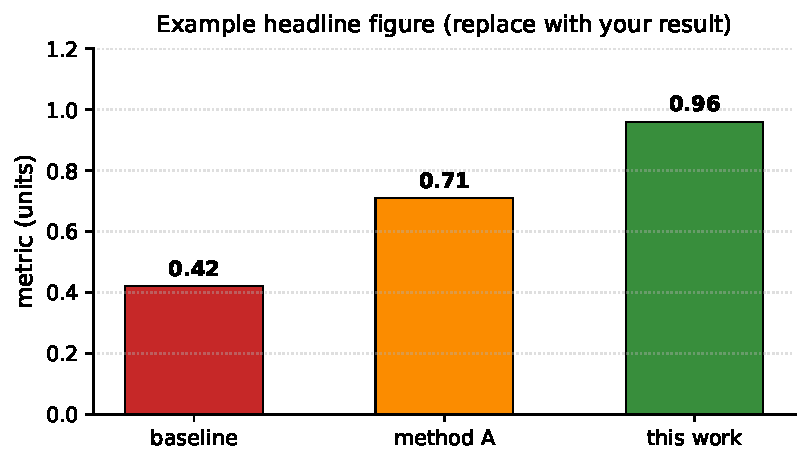
\includegraphics[width=0.7\linewidth]{figures/fig01_example.pdf}
\caption{Placeholder headline figure shipped with the template
(\texttt{figures/\_scripts/fig01\_example.py}). Replace the data, axes,
and this caption with your result. Captions carry the punchline first;
units must be explicit; error bars must be defined.}
\label{fig:headline}
\end{figure}

\begin{figure}[h]
\centering
\includegraphics[width=0.7\linewidth]{figures/fig02_line.pdf}
\caption{TikZ/pgfplots line example shipped with the template
(\texttt{figures/\_scripts/fig02\_line.tex}). Replace the line data with
your result; native LaTeX so no Python dependency.}
\label{fig:line}
\end{figure}

\begin{table}[h]
\centering
\small
\begin{tabular}{lcc}
\toprule
\textbf{Configuration} & \textbf{Metric} & \textbf{N} \\
\midrule
baseline       & 0.42 & 100 \\
method A       & 0.71 & 100 \\
this work      & 0.96 & 100 \\
\bottomrule
\end{tabular}
\caption{Placeholder results table. Replace rows with your headline
numbers; keep units in the column header and the caption.}
\label{tab:results}
\end{table}

\section{Limitations and honest caveats}
\label{sec:limits}

Enumerate what would invalidate the result and what is out of scope.
Each caveat should be specific enough that a reader can independently
judge whether it applies to their case.

\begin{itemize}\itemsep0.2em
\item Caveat 1: scope of the claim.
\item Caveat 2: parameter regime not swept.
\item Caveat 3: downstream wet-lab confirmation still \tierOrange.
\end{itemize}

\section{Reproducibility}
\label{sec:repro}

Code: \url{https://github.com/dancinlab/<repo>}. Data: \texttt{companion/}
(\texttt{verify-ledger.json}, \texttt{pr-roll.json},
\texttt{session-journal.md}, \texttt{adapter-defect-catalog.json}).
Build: \texttt{make} (xelatex \(\times 3\) + bibtex). Figures: \texttt{make figures}.
Word count: \texttt{make wordcount}. Page count: \texttt{make pages}.
Lint: \texttt{make lint}. Arxiv tarball: \texttt{make arxiv-tar}.

\section{Conclusion}
\label{sec:conclusion}

What this changes. What stays the same. The single most important
follow-up experiment.

% =========================================================================
\paragraph{Acknowledgments.}
This work used the \texttt{hexa-lang} verification surface and the
\texttt{sidecar/paper} scaffold. LLM collaborator credit (model + version,
e.g. Claude Opus 4.x) is listed here, not in the author block above.

% =========================================================================
\bibliographystyle{plainnat}
\bibliography{references}

% =========================================================================
% BLUE-MAX appendix template (commented out --- uncomment + fill when a paper
% does an algebraic-root audit that earns the BLUE-MAX badge).
%
% \appendix
% \section{BLUE-MAX appendix --- algebraic-root audit}
% \label{app:blue-max}
%
% Every claim in this paper is audited against the closed-form algebraic
% root below. Each row maps a claim to an `atom:<id>` whose verdict is
% \tierBlue\ (closed-form) or \tierGreen\ (numerical with proof).
%
% \begin{table}[h]
% \centering
% \small
% \begin{tabular}{@{}lll@{}}
% \toprule
% \textbf{Claim} & \textbf{Atom} & \textbf{Tier} \\
% \midrule
% claim 1 & \texttt{atom:<id-1>} & \tierBlue  \\
% claim 2 & \texttt{atom:<id-2>} & \tierGreen \\
% \bottomrule
% \end{tabular}
% \caption{BLUE-MAX audit table. Every paper claim has an atom; every
% atom has a verdict; no orange claims survive into the body.}
% \end{table}

\end{document}
